\documentclass{beamer}
\usepackage{graphicx}
\usepackage[catalan]{babel}
\usepackage[utf8]{inputenc}
\usepackage[T1]{fontenc}

\usetheme{Rochester}
\usecolortheme{wolverine}

\title{Què està passant a Perl 6}
\subtitle{La història de Perl, Rakudo i esdeveniments actuals}
\author{Tadeusz Sośnierz (autor original)\\
Alex Muntada (traducció al català)}

\begin{document}
\begin{frame}{Què està passant a Perl 6}
	\titlepage
\end{frame}

			\section{Introducció}

\begin{frame}{Per què parlem avui de Perl 6?}
	\begin{block}{Larry Wall}
		«Perl 5 was my rewrite of Perl. I want Perl 6 to be
		the community's rewrite of Perl
		and of the community.»
	\end{block}
	\pause
	\begin{itemize}
		\item 19 juliol 2000 -- anunci de Perl 6
			-- Fa exactament 10 anys!
		\pause
		\item Perl 6 no és només una especificació
		\pause
		\item En 10 dies (29 juliol) sortirà Rakudo Star
			-- una distribució de Perl 6 llesta per utilitzar
		\pause
		\item Aquest dijous (22 juliol) sortirà Rakudo \#31,
			en què es basarà Rakudo Star
	\end{itemize}
\end{frame}

\begin{frame}{Camelia}
	\begin{columns}
		\begin{column}{0.5\textwidth}
			
\includegraphics[scale=0.54]{camelia}
		\end{column}
		\begin{column}{0.5\textwidth}
			{\Huge »ö«}
		\end{column}
	\end{columns}
	
\includegraphics[scale=0.38]{newlogo}
\end{frame}

\begin{frame}{Rakudo i Parrot}
	\begin{center}
		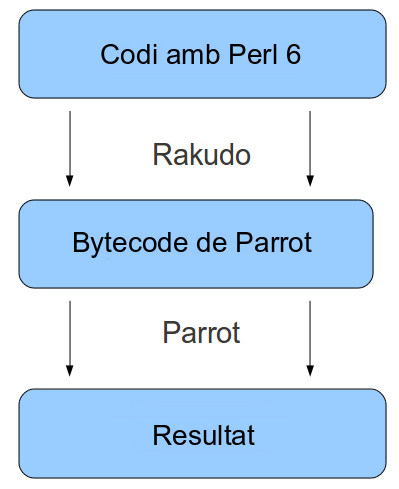
\includegraphics[scale=0.4]{bohomaz_ca}
	\end{center}
\end{frame}
			\section{Què està passant ara?}
			\subsection{Parrot}

\begin{frame}{Parrot}
	\begin{itemize}
		\item Una màquina virtual per a llenguatges dinàmics
		\item Implementacions disponibles per a Perl 6, Python, Ruby i altres
		\item Surt regularment cada mes, demà (20.07) la versió 2.6.0
	\end{itemize}
\end{frame}

			\subsection{Rakudo}

\begin{frame}{Rakudo}
	\begin{center}
		
\includegraphics[scale=0.5]{rakudo}
	\end{center}
	\begin{itemize}
		\item (Jap.) «The Way Of The Camel», o «Paradise»
		\item Compilador de Perl 6 en Perl 6
		\item També publicat cada mes, dos dies després que surti Parrot
		\item Actualment compleix el 83\% dels tests de les especificacions
	\end{itemize}
\end{frame}

\begin{frame}{Rakudo -- progrés}
	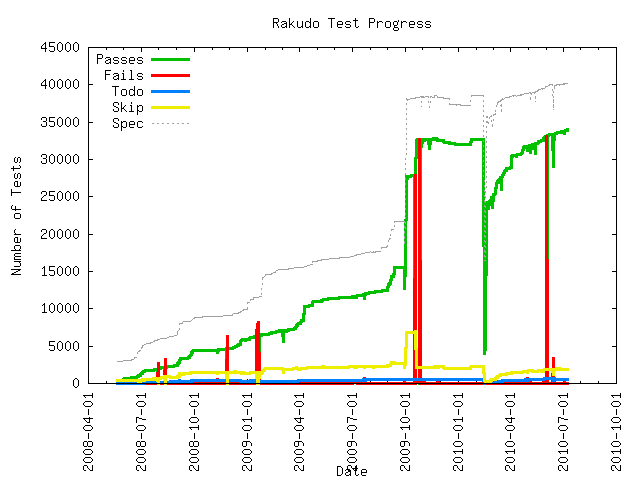
\includegraphics[scale=0.3785]{progress}
\end{frame}

			\subsubsection{Rakudo Star}

\begin{frame}{Rakudo Star}
	\begin{itemize}
		\item «useful and usable»
		\item Serà una implementació completa, però segura d'utilitzar
		\item Per atraure l'atenció i encoratjar la portabilitat dels mòduls i la programació
		\item Data planificada -- 29 juliol.
	\end{itemize}
\end{frame}

\begin{frame}{Rakudo Star}
	I juntament amb ell:
	\begin{itemize}
		\item Parrot
		\item Blizkost (en parlem tot seguit)
		\item Mòduls
		\begin{itemize}
			\item Zavolaj (native call interface)
			\item MiniDBI (subset DBI)
			\item ...
		\end{itemize}
	\item «The Perl 6 Book»
		(\htmladdnormallink{http://github.com/perl6/book}
		{http://github.com/perl6/book})
	\end{itemize}
\end{frame}

			\subsection{Relacionat}
\begin{frame}[fragile]{Blizkost}
	Permet la possibilitat d'utilitzar Perl 5 com un dels llenguatges
    a Parrot, que permet utilitzar mòduls de Perl 5 dins del codi
    en Perl 6
	\begin{block}{blikost/examples/cgi.pl}
\begin{verbatim}
use v6;
use CGI:from<perl5>;
my $q = CGI.new;

print $q.header, $q.start_html('Hello World'),
      $q.h1('Hello World'), $q.end_html;
\end{verbatim}
	\end{block}
\end{frame}

\begin{frame}[fragile]{Zavolaj}
	«Crida» una funció en C directament des de Perl 6
	\begin{block}{zavolaj/examples/sqlite3.p6 (fragments)}
\begin{verbatim}
use NativeCall;
sub sqlite3_open( Str $filename, OpaquePointer $ppDB )
    returns Int
    is native('libsqlite3')
    { ... }

my OpaquePointer $db;
my $status = sqlite3_open("test.db", $db);
\end{verbatim}
	\end{block}
\end{frame}

\begin{frame}{Mòduls -- proto, pls}
	\begin{itemize}
		\item proto -- instal·lador de mòduls de Perl 6
		\item projecte nou: pls (substitueix proto)
		\item \htmladdnormallink{http://modules.perl6.org}
			{http://modules.perl6.org} -- els mòduls base
		\begin{itemize}
			\item Math::Model
			\item MiniDBI
			\item LWP::Simple
			\item SVG
			\item ufo
			\item URI
			\item XML, XML::Writer
			\item Web
			\item HTTP::Server::Simple, HTTP::Server::Simple::PSGI (no disponibles en proto)
		\end{itemize}
	\end{itemize}
\end{frame}

\begin{frame}{Altres implementacions}
	\begin{itemize}
		\item PUGS (abandonat)
		\item YAPSI -- Yet Another Perl Six Implementation
			(\htmladdnormallink{http://github.com/masak/yapsi}
			{http://github.com/masak/yapsi})
		\item Niecza -- compilador de Perl 6 en .NET/Mono (\htmladdnormallink{http://github.com/sorear/niecza}{http://github.com/sorear/niecza})
		\item Bennu -- compilador del Perl 6 per a LLVM (\htmladdnormallink{http://github.com/ekiru/Bennu}{http://github.com/ekiru/Bennu})
	\end{itemize}
\end{frame}
			\section{Què ha canviat?}

\begin{frame}{Canvis, canvis, canvis}
	\begin{center}
	{\huge Què ha canviat al propi llenguatge?}
	\end{center}
\end{frame}

\begin{frame}{Què no agrada de Perl 5}
	\begin{itemize}
		\item OOP en cru
		\item Accés als paràmetres de les funcions
		\item Capturar excepcions
		\item Una sintaxi no gaire maca de vegades (referències)
	\end{itemize}
\end{frame}

\begin{frame}{Què ha canviat}
	\begin{itemize}
		\item OOP -- tot és un objecte, creant una nova sintaxi
			per a les classes (similar a la de MooseX::Declare)
		\item Expressions regulars, per una banda incompatibles
            amb les de Perl 5, però amb moltes més opcions
		\item Sintaxi -- s'han simplificat algunes coses,
			però se n'han afegit moltes d'altres
	\end{itemize}
\end{frame}

\begin{frame}[fragile]{Què ha canviat}
	\begin{center}
		{\Huge Però això encara és Perl}
	\end{center}
\end{frame}

\begin{frame}[fragile]{Quins mòduls ja no seran necessaris}
	% aquests són els que ja no calen perquè són part de l'estàndard
	\begin{itemize}
		\item Moose
		\item Try::Tiny
		\item Data::Dumper -- cada variable té un mètode .perl
		\item Devel::REPL -- els REPL tenen un estàndard
		\item Getopt::* -- es poden detectar els paràmetres per a
            la funció MAIN (això en un moment) %TODO
	\end{itemize}
\end{frame}
			\subsection{Comprovació de tipus}
\begin{frame}[fragile]{Comprovació de tipus}
	És possible assignar un tipus a una variable

	\begin{semiverbatim}
\alert{> my Int \$a = 5; \$a = "foo"}
Type check failed for assignment
	\end{semiverbatim}

	\begin{semiverbatim}
\alert{> my Str \$a = "foo"; \$a = 5}
Type check failed for assignment
# però...
\alert{> my Str \$a = "foo"; \$a = 5.Str; \$a.perl.say}
"5"
	\end{semiverbatim}
	\begin{semiverbatim}
\alert{> say ~[5.WHAT, 'string'.WHAT, (3/7).WHAT, /foo .*/.WHAT]}
Int() Str() Rat() Regex()
	\end{semiverbatim}
\end{frame}

			\subsection{Tot és un objecte}

\begin{frame}[fragile]{Tot és un objecte}
	\begin{semiverbatim}
\alert{> 'a string'.\^\relax{}methods.sort[40..45]}
bytes can capitalize ceiling chars chomp
\alert{> "the big brown fox".split(' ').grep(/\^\relax{}b/).join(' and ')}
big and brown
	\end{semiverbatim}
\end{frame}
			\subsection{Prefixos de variables}
\begin{frame}{Prefixos de variables}
		A Perl 6 el prefix d'una variable (sigil) no canvia durant l'extracció d'un sol element
	\vskip15pt
	\begin{tabular}{l|l}
	Perl 5 & Perl 6 \\
	\hline
	\hline
	my @arr = (1, 2, 3) & my @arr = (1, 2, 3) \\
	my \$elem = \alert{\$arr}[1] & my \$elem = \alert{@arr}[1] \\
	\hline
	my \%hash = (foo => 'bar') & my \%hash = (foo => 'bar') \\
	my \$elem = \alert{\$hash}\{'foo'\} & my \$elem = \alert{\%hash}\{'foo'\} \\
	\end{tabular}
\end{frame}
			\subsection{Tot és una referència}
\begin{frame}[fragile]{Tot és una referència}
	No hi ha distinció entre variables i referències cap a elles,
    d'aquesta manera no hi ha problemes de dereferenciació.
	\begin{verbatim}
my $a = [ { foo => [1, 2, 3] } ];
	\end{verbatim}
	\begin{columns}[t]
		\begin{column}{0.5\textwidth}
			\begin{block}{Perl 5}
				\begin{verbatim}
say $a->[0]->{foo}->[1] # 2
				\end{verbatim}
			\end{block}
		\end{column}
		\begin{column}{0.5\textwidth}
			\begin{block}{Perl 6}
				\begin{verbatim}
say $a[0]<foo>[1] # 2
				\end{verbatim}
			\end{block}
		\end{column}
	\end{columns}
\end{frame}
			\subsection{Funcions i paràmetres}
\begin{frame}[fragile]{Funcions i paràmetres}
	\begin{verbatim}
sub foo (Str $what, Int $times = 1) {
    say $what x $times
}

foo "hello", 5; # hellohellohellohellohello
foo "hello";    # hello
foo;            # Not enough positional parameters passed;
                # got 0 but expected between 1 and 2
	\end{verbatim}
\end{frame}
			\subsection{La funció MAIN}
\begin{frame}[fragile]{La funció MAIN}
\small
\begin{verbatim}
sub MAIN($v?, :$arg!, :$arg2 = 'predeterminat') {
    if ($v) { # verbose
        say "Inici"
    }
    say "arg: $arg, arg2: $arg2"
}
\end{verbatim}
\begin{semiverbatim}
\$ \alert{perl6 main.pl}
Usage:
./main.pl [--arg2=value-of-arg2] --arg=value-of-arg [v]

\$ \alert{perl6 main.pl -v --arg=5}
Inici
arg: 5, arg2: predeterminat

\$ \alert{perl6 main.pl --arg=5 --arg2=foo}
arg: 5, arg2: foo
\end{semiverbatim}
\end{frame}
			\subsection{Junctions}
\begin{frame}[fragile]{Junctions}
	\begin{semiverbatim}
\alert{> say 'ok' if 5 == any(3, 5, 7) # albo 5 == 3 | 5 | 7}
ok
\alert{> say 'ok' if 5 == none(4, 6, 8)}
ok
\alert{> my Junction \$x = 3 | 5; say 'ok' if \$x == 5}
ok
\alert{> my @scores = 32, 41, 73, 99, 52;
> say 'ok' if all(@scores) > 30;}
ok
	\end{semiverbatim}
\end{frame}
			\subsection{Laziness}
\begin{frame}[fragile]{Laziness}
	\begin{semiverbatim}
\alert{> my \$even = (2, 4 ... *); \$even[\^\relax{}10].perl.say}
(2, 4, 6, 8, 10, 12, 14, 16, 18, 20)
\alert{> my \$sq = gather for 0..Inf \{ take \$\_ * \$\_ \}; \$sq[5].say}
25
	\end{semiverbatim}
\end{frame}
			\subsection{Try-CATCH}
\begin{frame}[fragile]{Try-CATCH}
\begin{verbatim}
try {
    die "Oh noes!";
    CATCH {
        say "Something went wrong: $_";
    }
}
\end{verbatim}
\end{frame}
			\subsection{OOP -- Perl 6 i Moose}
\begin{frame}[fragile]{OOP}
\begin{columns}[t]
	\begin{column}{0.5\textwidth}
	\begin{block}{Perl 5 amb Moose}
{\tiny
\begin{verbatim}
package Point;
use Moose;

has ['x','y'] => (is => 'rw', isa => 'Int');

sub clear {
    my $self = shift;
    $self->x(0);
    $self->y(0);
}

package Point3D;
use Moose;
extends 'Point';

has 'z' => (is => 'rw', isa => 'Int');

after 'clear' => sub {
    my $self = shift;
    $self->z(0);
};
\end{verbatim}
}
	\end{block}
	\end{column}
	\begin{column}{0.5\textwidth}
	\begin{block}{Perl 6}
{\tiny
\begin{verbatim}
class Point {

  has Int $.x is rw;
  has Int $.y is rw;

  method clear {
    $.x = $.y = 0;
  }

}

class Point3D is Point {

  has Int $.z is rw;

  method clear {
    nextsame;
    $.z = 0;
  }

}
\end{verbatim}
}
	\end{block}
	\end{column}
\end{columns}
\end{frame}
			\subsection{Gramàtiques}
\begin{frame}[fragile]{Gramàtiques}
\tiny
\begin{verbatim}
grammar URI {
    token TOP {
        <schema> '://'
        [<hostname> | <ip> ]
        [ ':' <port>]?
        '/' <path>?
    }
    token byte {
        (\d**{1..3}) <?{ $0 < 256 }>
    }
    token ip {
        <byte> [\. <byte> ] ** 3
    }
    token schema {
        \w+
    }
    token hostname {
        (\w+) ( \. \w+ )*
    }
    token port {
        \d+
    }
    token path {
        <[ a..z A..Z 0..9 _\-.!~*'():@&=+$,/ ]>+
    }
}
my $match = URI.parse('http://perl6.org/documentation/');
say $match<hostname>;  # perl6.org
say $match<path>;      # documentation
\end{verbatim}
\end{frame}

			\section{I ara què?}
\begin{frame}{Què podem fer ara}
	Què podem fer mentre esperem a Rakudo Star?
	\begin{itemize}
		\item Escriure codi per detectar errors
		\item Fer soroll positivament sobre Perl 6 :)
	\end{itemize}
\end{frame}
			\section{Enllaços}

\begin{frame}{Enllaços}
	\begin{itemize}
		\item \htmladdnormallink{http://perl6.org/}
			{http://perl6.org/}
		\item \htmladdnormallink{http://parrot.org/}
			{http://parrot.org/}
		\item \htmladdnormallink{http://rakudo.org/}
			{http://rakudo.org/}
		\item
		\htmladdnormallink{http://perlgeek.de/en/article/5-to-6}
		{http://perlgeek.de/en/article/5-to-6}
		-- introducció a Perl 6 per a programadors de Perl 5
		
		\item \htmladdnormallink{http://perl6advent.wordpress.com/}
			{http://perl6advent.wordpress.com/}
			-- Perl 6 Advent Calendar, una sèrie d'articles
            interessants amb notícies sobre Perl 6
		\item El canal \#perl6 a irc.freenode.net
	\end{itemize}
\end{frame}

\end{document}
